\documentclass[11pt]{article}
\usepackage[utf8]{inputenc}
\usepackage{amsmath}
\usepackage{titlesec}
\usepackage{titling}
\usepackage{geometry}
\usepackage{graphicx}
\usepackage{hyperref}
\usepackage{fancyhdr}
\usepackage{wallpaper}
\usepackage{afterpage} 
\usepackage{pagecolor} 
\usepackage[nottoc]{tocbibind} % Put the bibliography in the ToC
\usepackage{url}
\usepackage[toc,page]{appendix}

% Define colors
\usepackage{xcolor}
\definecolor{myblue}{RGB}{33, 66, 99}
\definecolor{mygray}{RGB}{169, 169, 169}
\definecolor{darkbluegrey}{RGB}{44, 62, 80} 

% Page styling
\pagestyle{fancy}
\fancyhf{}
\renewcommand{\headrulewidth}{0pt}
\renewcommand{\footrulewidth}{0pt}
\fancyfoot[C]{\thepage}
\renewcommand{\familydefault}{\sfdefault}

% Define a command for section headers
\titleformat{\section}
  {\color{myblue}\normalfont\Large\bfseries}
  {\color{myblue}\thesection}{1em}{}

% Define a command for subsection headers
\titleformat{\subsection}
  {\color{myblue}\normalfont\large\bfseries}
  {\color{myblue}\thesubsection}{1em}{}

% Adjust page margins
\geometry{a4paper, margin=1in}

% make references clickable
\hypersetup{
    colorlinks=true,
    linkcolor=blue,
    filecolor=magenta,      
    urlcolor=cyan,
}

\begin{document}

% Change the background color of the first page
\pagecolor{darkbluegrey}
\afterpage{\nopagecolor}

% Add a background image
\ThisCenterWallPaper{0.75}{./image/bi.png}

\begin{titlepage}
  \vspace*{\stretch{1}}
  \begin{center}
    \textcolor{white}{\textbf{\Huge Description of Work}}\\ % changed text color to white
    \vspace{1cm}
    \textcolor{white}{\Large Sound Detection and Classification\\using Spiking Neural Networks} % changed text color to white
    \vspace{3cm}
  \end{center}
  \vspace*{\stretch{2}}
  \begin{center}
    \textcolor{white}{ % changed text color to white
      \textbf{COURREGE Téo}\\
      \textbf{GANDEEL Lo'aï}\\
      \vspace{1cm}
      \Large Date: \today}
  \end{center}
  \vspace*{\stretch{1}}
\end{titlepage}

\newpage

\tableofcontents

\pagebreak

\section{Introduction}

In the constantly evolving landscape of neural network studies, the project outlined in this Description of Work (DoW) proposes to explore the field of spiking neural networks (SNNs). This effort will at term combine both a study and a prospective implementation, with a focus on the emerging field of neuromorphic computing.

The overall goal of this project is to perform a thorough investigation and subsequent implementation of spiking neural networks. SNNs, which are inspired by the neural signaling patterns of the human brain, show promising potential in various applications, especially in real-time processing and pattern recognition.

Before getting into the specifics of our project, let us first give a brief overview of what spiking neural networks are and how they work:

A Spiking Neural Network (or SNN) is a type of artificial neural network that mimics the functionality of biological neural networks. Unlike traditional neural networks (ANNs - Artificial Neural Networks), SNNs incorporate the concept of time into their operating model. The neurons in SNNs generate spikes of activity and communicate through these spikes (like brain neurons stimulating each other with electrical impulses), allowing them to process information in a more complex and potentially more efficient manner.

This type of neural network is theoretically less energy consuming than some ANNs and potentially more efficient in terms of processing power (in practice, it will be necessary to create an adapted hardware architecture to take advantage of this potential). Therefore, it seems that the use of this type of neural network could be a viable solution to a classification processing problem (especially in real time ones).

Our project focuses on a specific problem within the broader domain of audio classification.

Adopting an exploratory approach, we will begin this DoW with a more detailed presentation of the dataset used and its construction. After a brief introduction of our topic, we will review the state of the art in the field of SNNs and audio classification. We will then present the technical goals of our project and a simple theoretical study of SNNs. Finally, we will present the resources we have at our disposal to carry out this project, as well as a description of the work to be done. Finally, we will propose a schedule for the project.



\section{Chosen theme}
\subsection{The SNN}
\subsubsection{Definition}
Spiking Neural Network (SNN) is a variant of artificial neural network that try to mimic more closely the biological neural networks. More precisely, it tries to copy the functioning of neurons and synapses. As a result, rather than working with continually changing time values as ANNs do, SNNs work with discrete events that happen at defined times. SNNs take a set of spikes as input and produces a set of spikes as output

\begin{figure}[h]
  \centering
  \begin{minipage}{0.45\textwidth}
    \centering
    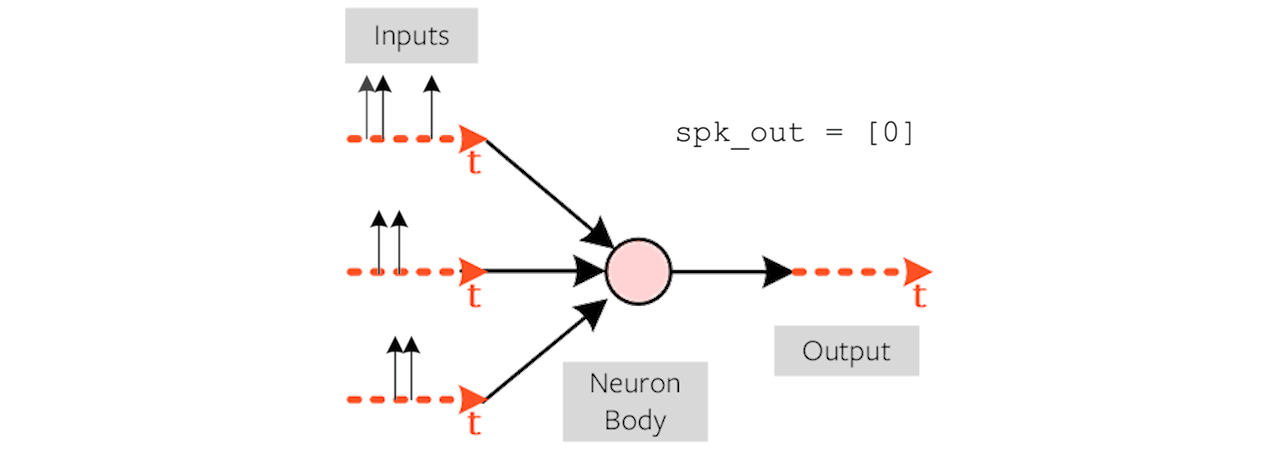
\includegraphics[width=1\textwidth]{image/def1.png}
  \end{minipage}\hfill
  \begin{minipage}{0.45\textwidth}
    \centering
    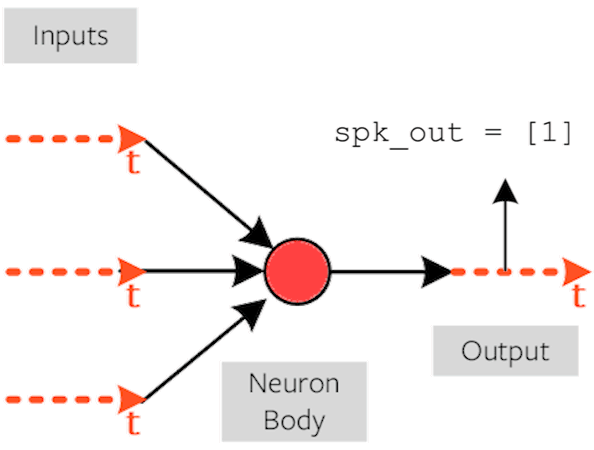
\includegraphics[width=1\textwidth]{image/def2.png}
  \end{minipage}
\end{figure}


The spiking behavior of a neuron in an SNN is modeled by the membrane potential equation:
$$
  V(t) = \sum_{i} W_i \cdot \delta(t - t_i)
$$

Here, \(V(t)\) is the membrane potential, \(W_i\) is the synaptic weight, and \(\delta(t - t_i)\) is the Dirac delta function representing the occurrence of a spike at time \(t_i\).

The output spikes \(Y\) can be obtained based on a threshold \( \theta \):
$$
  Y(t) =
  \begin{cases}
    1 & \text{if } V(t) \geq \theta \\
    0 & \text{otherwise}
  \end{cases}
$$

\subsubsection{Advantages / Disadvantages}


SNNs, when well constructed, should offer the following benefits:

- Energy efficiency: SNNs are highly energy efficient because they only consume energy when a spike is generated, unlike "classical" neural networks which consume energy continuously. This makes them ideal for low-power embedded devices.

- Event-driven processing: While ANNs typically operate on a fixed time interval, SNNs only process information when there is an input spike. This makes them highly efficient at processing information in an event-driven environment, such as processing visual or audio data.

- Temporal coding: SNNs are able to process information based on the timing of spikes, allowing them to encode temporal information and be temporally accurate. This is particularly useful for tasks that require the processing of sequential data, such as speech or gesture recognition.

- Robustness to noise: SNNs are inherently robust to noise and can effectively filter out irrelevant information. This makes them useful in environments where noise is a common problem, in our case it may be an instance of audio not well recorded.

- Neuroplasticity: SNNs are able to adapt to new inputs and change their behaviour over time, much like the brain. This allows them to learn and adapt to new tasks and environments, making them highly versatile.


Disadvantages:

- SNNs are difficult to train, mainly due to backpropagation issues, which are caused by the discrete, temporal nature of spikes. Backpropagation in time (BPTT) is the typical method used, but it suffers from issues such as the temporal credit assignment problem (the determination of which past events or actions contributed most significantly to the current outcome or state)

- There is currently no learning algorithm designed specifically for this task, SNNs lacks the "maturity" of more classic neural networks.

- Building a small SNN is impractical. Indeed, we need a sufficient number of neurons to retrieve useful informations.

We will try to highlight these specificities during our project

\subsubsection{snnTorch}
We will primarily work in Python and use the \hyperref[item:snntorch-lib]{snnTorch} package to work on SNNs. snnTorch is a Python package for performing gradient-based learning with spiking neural networks. snnTorch is built on top of Pytorch and takes advantage of its GPU-accelerated tensor computation. Pre-defined spiking neuron models are integrated into the PyTorch framework and can be treated as recurrent activation units.


\subsection{Neural networks applied to audio classification}
\subsubsection{Definition}
Audio classification is a machine learning and signal processing task that involves categorizing or labeling audio data into different predefined classes or categories. The goal is to automatically assign a label to an audio segment based on its content or characteristics. This can be useful in various applications :

-Speech Recognition: Identifying spoken words or phrases in audio recordings.

-Music Genre Classification: Categorizing music into different genres, such as rock, pop, jazz, etc.

-Environmental Sound Analysis: Detecting and classifying sounds in the environment, such as sirens, footsteps, or car engines.

-Anomaly Detection: Identifying unusual or unexpected sounds in a given context.

\subsubsection{How it works}

The process of audio classification is relatively similar to image classification and typically involves the following steps

Data collection: Collecting a dataset of audio samples, each labeled with its corresponding class or category.

Feature extraction: Transforming the raw audio data into a set of relevant features that can be used to represent the content of the audio. Common features include spectrogram representations, Mel Frequency Cepstral Coefficient, and other time or frequency domain features.

Model training: Using machine learning algorithms or deep learning architectures to train a model on the extracted features and their corresponding labels. Apart from neural networks, others algorithms can be used for audio classification such as support vector machines, decision trees, or random forests for example.

Validation and testing: Evaluate the performance of the trained model on a separate set of data that it has not seen before. This helps evaluate the model's ability to generalize to new, unseen examples.

Deployment: Integrate the trained model into applications or systems that require real-time or batch audio classification.

\subsection{Relevance of this choice}
\subsubsection{Defining the project's pros and cons}
Pros :
\begin{itemize}
  \item SNN's can be effective to detect and recognize different types of audio (especially on embedded devices).
  \item The comparison between SNN and other types of neural networks will be particularly important to us, and we will try to show what can be the strengths and drawbacks of SNNs compared to other networks.
\end{itemize}

Cons:

\begin{itemize}
  \item SNNs are new to us, we need to understand the package snnTorch.
  \item Training SNNs is harder,
\end{itemize}

\subsubsection{Cases of use to define the relevance of the project}
Our final goal is primarily to compare the efficiency and energy use of SNNs compared to others networks (CNNs, RNNs, LSTMs...) in audio classification, and to evaluate if SNNs are a good solution in our case.



\section{Data used}
\subsection{Choosing the type of training data}

When we first read the survey about $SNNs^{\cite{snn_survey}}$, it was understood that training this type of model would be more difficult than some ANNs due to the temporal dynamics involved in SNNs. This made us want to work on a type of data that would be less computationally or resource intensive than videos (so that we could store and train our models on many of them). This type of data also has the advantage of being more adaptable to pre-recorded and real-time processing.
\subsection{Feasibility}

In our case, we decided to apply our analysis to the \hyperref[item:google-audioset]{Google AudioSet} database, which contains a large number of audio samples classified into different categories.
The structure of this dataset is as follows: each audio sample is associated with a label, and each label is associated with a set of audio samples. In practice, this dataset is composed of '.csv' files that contain one or more labels, a timecode (10 seconds of duration), and a part of an url that would help us find an associated Youtube video. This gave us 2 problems: a copyright problem and the fact of extracting the data and formatting it in a way that would be usable for our project.

\subsubsection{Copyright}

According to \hyperref[item:google-audioset]{the AudioSet website} (download page): "The dataset is made available by Google Inc. under a Creative Commons Attribution 4.0 International (CC BY 4.0) license, while the ontology is available under a Creative Commons Attribution-ShareAlike 4.0 International (CC BY-SA 4.0) license".


\subsubsection{Data collection/extraction}

Fortunately for us, we found \hyperref[item:google-audioset-reformatted]{some GitHub repositories} whose code aims to download, format, and crop the various sound files so that it "unifies the formats of the datasets so that it is possible to analyze them in the same pipelines". The given script also included a parallelization of the calculation.

After some slight modifications we were able to check the impact on memory resources, for example for \href{https://www.youtube.com/watch?v=dQw4w9WgXcQ}{this youtube video} we get

\begin{itemize}
  \item Resource usage (RAM, GPU, CPU, time)
        \subitem Size of 144p: 2-4 MB (depending on format)
        \subitem Size of the same video as an audio file (wav in best quality): 1-3 MB (depending on the format)
\end{itemize}

Without parallelizing the code we used, we were able to download, format, and trim 6 audio files in about 60 seconds (and our first attempts at parallelizing seemed promising, though there are still bugs to work out). At this pessimistic rate, we think we should be able to download, format and trim about 2000 10-second audio files in about 5-6 hours. By limiting the number of labels to study to about ten, we think we might get some results (to be tested with a pre-trained Pytorch model).

\subsubsection{Uncertainties about data quality}

While lookin up to the data, we found that a lot of these sounds are taken out of context and other sounds are mixed with them (for example, \hyperref{https://www.youtube.com/watch?v=-0CamVQdP_Y}{}{}{this} sample is labeled with as a music sound but a person is talking at the end of the sample). Also, each sample can have one or multiple labels, which can be related to multi-clustering problems.
Another problem we face is the fact that the data is always balanced (there exists a balanced version of the dataset) and that there are some Weak and Strong Label annotations.

Strong labels are precise and indicate the exact start and end times of the event in the audio file whereas the Weak labels, only indicate the presence of a sound event somewhere in the audio file, without specifying the exact time. 

\subsection{Open to other databases}

\section{State of the art}
\subsection{Finding what already exists}
\subsubsection{In a simple neural network}
\paragraph{Trained on the same data set or not}
\subsubsection{In SNN}
\paragraph{Trained on the same data set or not}
\subsubsection{Existing libraries, existing models}
\subsection{Results obtained as a basis for comparison}

\section{Technical objectives of the project}
\subsection{Technical objectives achievable with pre-existing ANNs}




\subsection{Technical objectives with data}
{\color{blue}
  How AI and ML Understand and Classify Audio

  In its raw form, a sound is an analog signal — to process it, we have to convert it to digital. Analog signals are continuous waves. An analog wave has a discrete value at any given point in time. It’s impossible to convert every value to a digital representation because there are infinite points in a continuous wave. You must convert the audio signal to digital through sampling and quantization.

  Sampling means recoding these points at specific time intervals or frequencies. This interval is the sample rate. The higher the sample rate, the less information lost and the fewer errors. However, if the sample rate is too high, it increases the audio file size without significantly improving the audio.

  Quantization means rounding the amplitude sampled at each interval to the nearest bit. The greater the bit depth, the lower the quantization. The larger the bit depth, the more memory it takes, so what bit depth to use depends on the amount of available RAM. If you want to learn more, this is a good explanation of analog to digital conversion.

  After conversion, the next step is to extract useful features from the audio. You can extract many features, so you must focus on the specific problem you want to solve. Here are some critical features used for audio classification with ML:

  Time domain features are extracted directly from the raw audio (waveform). Examples are the amplitude envelope, and the root mean square energy. Time domain features are not enough to represent the sound because they do not include frequency information.

  Frequency domain features are also called the spectrum. Examples include band energy ratio, spectral flux, and spectral bandwidth. These features lack time representation. You extract them from a time domain representation through Fourier transform. Fourier transform converts a waveform from a function of time to a function of frequency. Learn more about Fourier Transforms here.

  Time and frequency domain features extract a spectrogram from the waveform using a short-time Fourier transform, like Spectrogram or Mel Spectrogram. The spectrogram shows both the frequency and time domain. Spectrograms represent frequency linearly, but humans perceive sounds logarithmically. This means that humans can tell the difference between lower frequencies like 500-100 Hertz (Hz) but find it harder to differentiate between sounds at a higher frequency, from 10,000 Hz to 15,000 Hz. Learn more about how humans respond to various sound ranges here. This difficulty is why the Mel-scale was introduced. A Mel Spectrogram is a spectrogram on the Mel-scale, which measures how different pitches sound to the listener. It maps pitches that, to listeners, sound equidistant.

}


\subsection{Technical objectives with SNNs}
\subsection{Feasibility}
\subsubsection{Describing uncertainties}
Uncertainty are due to the dynamic nature of audio signals, varying acoustic environments, and the complexity of distinguishing between diverse sound patterns. Additionally, challenges in precisely modeling the temporal aspects of auditory processing and the understanding of spiking neuron dynamics contribute to many uncertainties in the feasibility of the project. Moreover the training of Spiking Neural Networks in order to attain a good accuracy is difficult due to the inherent non- linearity and sparsity of spikes.


\subsubsection{Looking for a working model}

Many model for sound classification already exist. In particular, for AudioSet, there are already multiple pre-trained deep neural network, for example YamNet. However, it is more difficult to find open source SNNs, as they are less widespread than other types of neural networks.


\subsubsection{Estimate computation time}



\section{Theoretical study}
\subsection{Theoretical study on SNN}


We will need to choose multiple parameters regarding our neural network, like the encoding and the type of training.

Neural coding schemes are used to convert input pixels into spikes that are transmitted to the excitatory neurons. There are four main neural coding schemes: rate coding, time-to-first spike coding, phase coding, and burst coding.



There are also multiple ways to train a SNN:

• Shadow training: A non-spiking ANN is trained and converted into an SNN by interpreting the activations as
a firing rate or spike time

• Backpropagation using spikes: The SNN is natively trained using error backpropagation, typically through
time as is done with sequential models

• Local learning rules: Weight updates are a function of signals that are spatially and temporally local to the
weight, rather than from a global signal as in error backpropagation



\section{Matching with available resources}
\subsection{Work time}

data collection/extraction:

- from csv/Youtube to mp3 : 1-2 days

data preprocessing:

-data cleaning/enhancement/augmentation: 3-4

models implementation:

-understanding snnTorch basic: 1-2 days

-finding pretrained/creating and tuning models: 4 days

training/tuning:

- training: weeks

- extracting information: weeks

working on the DOWs and presentation:

- DOWs writing: continous work, 1-2 hours each day

- slides for oral presentation: 2-3 days

\subsection{Computer resources}

Hardware: 2 laptops

Software: Google Colab (primarily)

\subsection{Human resources}

We will work in parallel most of the time, each one focusing on a different aspect to gain time when it is possible.

\pagebreak

\section{Appendix}

\subsection{Data}

\subsubsection*{Data Set used for the project}

\begin{itemize}
  \item Google AudioSet : \url{https://research.google.com/audioset/}
        \label{item:google-audioset}

\end{itemize}



\subsection{Code}

\begin{itemize}
  \item Sparsity through Spiking Convolutional Neural Network (SCNN) for Audio Classification at the Edge : \url{https://github.com/CongSheng/SpikingConvNN-AudioClassification/tree/main}
        \label{item:SCNN-audio-classification}
  \item Multilayer Spiking Neural Network for audio samples classification using SpiNNaker : \url{https://github.com/jpdominguez/Multilayer-SNN-for-audio-samples-classification-using-SpiNNaker}
        \label{item:spinnaker-audio-classification}

\end{itemize}

\subsection{Links}

\pagebreak

% Bibliography
\bibliographystyle{siam}
\bibliography{ref}

\end{document}
